\documentclass{article}
\linespread{1.3}
\usepackage[margin=50pt, headheight=100pt, headsep=5pt]{geometry}
\usepackage{amsmath, amssymb, amsthm, tikz, fancyhdr, float, graphicx, spverbatim, systeme}
\pagestyle{fancy}
\renewcommand{\headrulewidth}{0pt}
\newcommand{\changefont}{\fontsize{15}{15}\selectfont}

\fancypagestyle{firstpageheader}{
  \fancyhead[R]{
    \changefont
    \parbox[t]{4cm}{ % Adjust width as needed
      Michael Huang\\
      EN.625.740.81\\
      Homework 11
    }
  }
}
\begin{document}
\thispagestyle{firstpageheader}
{\Large

The file \verb|hw_11_data.txt| containts training data in three columns \(\{\mathbf{x_1}, \mathbf{x_2}, \mathbf{c}\}\) for two clusters, where \(\mathbf{c}\) is the cluster label. The data is not linearly separable.

}
{\Large 

\section*{1.}

Write code to implement a perceptron, with inputs 
\[
  z+0 = 1, z_1 = x_1, z_2 = x_2, z_3 = x^2_1, z_4 = x^2_2, z_5 = x_1 x_2
\]
I got the following results:
\begin{spverbatim}
> python problem_1.py
Learned weights [w0, w1, w2, w3, w4, w5]: [-7.82 -4.59  0.54 -0.34  1.25 -0.21]
Training accuracy: 100.00%
\end{spverbatim}
As a result of running the following code in a python script:
\begin{spverbatim}
import numpy as np 

training_data = np.loadtxt("hw_11_data.txt", delimiter=",")
x_1 = training_data[:, 0]
x_2 = training_data[:, 1]
c = training_data[:, 2]
# Translate labels to {-1, 1}
y = np.where(c == 1, 1, -1)

# z + 0 = 1, z_1 = x_1, z_2 = x_2, z_3 = x_1^2, z_4 = x_2^2, z_5 = x_1 x_2
Z = np.column_stack([
  np.ones_like(x_1),
  x_1,
  x_2,
  x_1 ** 2,
  x_2 ** 2,
  x_1 * x_2,
])

w = np.zeros(Z.shape[1])
eta = 0.01

for _ in range(1000):
  error_count = 0
  for i in range(len(y)):
    if y[i] * np.dot(w, Z[i]) <= 0:
      w += eta * y[i] * Z[i]
      error_count +=1
  if error_count == 0:
    break

accuracy = np.mean(np.where(np.dot(Z, w) >= 0, 1, -1) == y)
print("Learned weights [w0, w1, w2, w3, w4, w5]:", np.round(w, 2))
print(f"Training accuracy: {(accuracy * 100):.2f}%")
\end{spverbatim}

}
{\Large 

\section*{2.}

Implement a linear support vector machine in the \(\{x_1, x_2\}\) space. \\ \\
I got the following results:
\begin{verbatim}
> python problem_2.py
Linear SVM Accuracy: 82.50%
Weights ([w_1, w_2]): [-0.54  0.03]
Intercept (w_0): -0.33
\end{verbatim}
As a result of running the following code in a python script:
\begin{verbatim}
import numpy as np
from sklearn.svm import SVC

training_data = np.loadtxt("hw_11_data.txt", delimiter=",")
x_1 = training_data[:, 0]
x_2 = training_data[:, 1]
X = np.column_stack([x_1, x_2])
c = training_data[:, 2]
# Translate labels to {-1, 1}
y = np.where(c == 1, 1, -1)

linear_svm = SVC(kernel="linear").fit(X, y)
linear_svm_accuracy = linear_svm.score(X, y)
print(f"Linear SVM Accuracy: {(linear_svm_accuracy * 100):.2f}%")
print("Weights ([w_1, w_2]):", np.round(linear_svm.coef_[0], 2))
print("Intercept (w_0):", np.round(linear_svm.intercept_[0], 2))
\end{verbatim}

}
{\Large 

\section*{3.}

Implement a linear support vector machine in the \(\{z_1, z_2, \dots z_5\}\) space. Map back into the \(\{x_1, x_2\}\) space, and plot the resulting boundary. \\ \\
I got the following results: \\ \\ \\
\begin{verbatim}
> python problem_3.py
Linear SVM for Z Accuracy: 100.00%
Weights ([w_1, w_2, w_3, w_4, w_5]): [ 0.   -2.81  0.08  0.03  0.71 -0.01]
Intercept (w_0): -5.61
\end{verbatim}
\begin{figure}[h!]
  \centering
  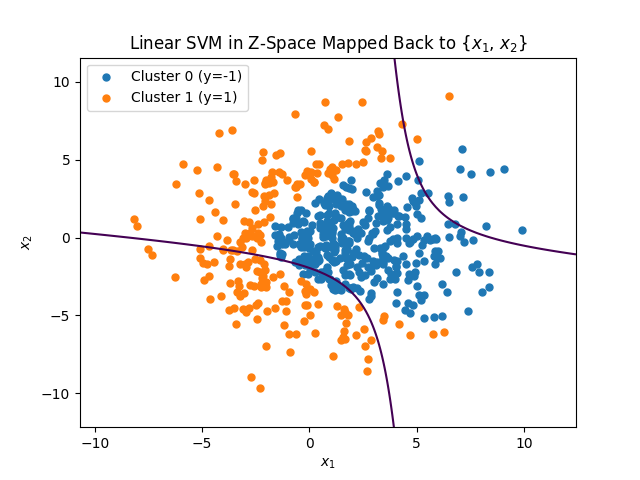
\includegraphics[width=500pt]{problem_3_contour.png}
\end{figure} 
As a result of running the following code in a python script:
\begin{verbatim}
import matplotlib.pyplot as plt
import numpy as np
from sklearn.svm import SVC

training_data = np.loadtxt("hw_11_data.txt", delimiter=",")
x_1 = training_data[:, 0]
x_2 = training_data[:, 1]
X = np.column_stack([x_1, x_2])
c = training_data[:, 2]
# Translate labels to {-1, 1}
y = np.where(c == 1, 1, -1)

# z + 0 = 1, z_1 = x_1, z_2 = x_2, z_3 = x_1^2, z_4 = x_2^2, z_5 = x_1 x_2
Z = np.column_stack([
  np.ones_like(x_1),
  x_1,
  x_2,
  x_1 ** 2,
  x_2 ** 2,
  x_1 * x_2,
])

z_svm = SVC(kernel="linear").fit(Z, y)
z_svm_accuracy = z_svm.score(Z, y)
print(f"Linear SVM for Z Accuracy: {(z_svm_accuracy * 100):.2f}%")
w = z_svm.coef_[0]
w_0 = z_svm.intercept_[0]
print("Weights ([w_1, w_2, w_3, w_4, w_5]):", np.round(w, 2))
print("Intercept (w_0):", np.round(w_0, 2))

# Grid for plotting the boundary 
x_1_grid = np.linspace(x_1.min() - 2.5, x_1.max() + 2.5, 100)
x_2_grid = np.linspace(x_2.min() - 2.5, x_2.max() + 2.5, 100)
X_1, X_2 = np.meshgrid(x_1_grid, x_2_grid)

# Map back into {x1, x2} space
f = (
  w_0
  + w[0] * X_1
  + w[1] * X_2
  + w[2] * (X_1 ** 2)
  + w[3] * (X_2 ** 2)
  + w[4] * (X_1 * X_2)
)

plt.scatter(x_1[c == 0], x_2[c == 0], label="Cluster 0 (y=-1)", s=25)
plt.scatter(x_1[c == 1], x_2[c == 1], label="Cluster 1 (y=1)", s=25)
plt.contour(X_1, X_2, f, levels=[0])
plt.xlabel("$x_1$")
plt.ylabel("$x_2$")
plt.title("Linear SVM in Z-Space Mapped Back to {$x_1$, $x_2$}")
plt.legend()
plt.show()
\end{verbatim}

}
{\Large 

\section*{4.}

Implement a support vector machine with a polynomial kernel. \\ \\
I got the following results:
\begin{verbatim}
> python problem_4.py
Polynomial Kernel SVM Accuracy: 100.00%
Number of support vectors: 10
\end{verbatim}
As a result of running the following code in a python script:
\begin{verbatim}
import numpy as np
from sklearn.svm import SVC

training_data = np.loadtxt("hw_11_data.txt", delimiter=",")
x_1 = training_data[:, 0]
x_2 = training_data[:, 1]
X = np.column_stack([x_1, x_2])
c = training_data[:, 2]
# Translate labels to {-1, 1}
y = np.where(c == 1, 1, -1)

# To fit K(x, x') = (1 + <x, x'>)^d
poly_svm = SVC(kernel="poly", degree=2, gamma=1, coef0=1).fit(X, y)
poly_svm_accuracy = poly_svm.score(X, y)
print(f"Polynomial Kernel SVM Accuracy: {(poly_svm_accuracy * 100):.2f}%")
print("Number of support vectors:", len(poly_svm.support_))
\end{verbatim}

}
{\Large 

\section*{5.}

Implement a support vector machine with a radial basis function kernel. \\ \\
I got the following results:
\begin{verbatim}
> python problem_5.py
Radial Basis Function Accuracy: 99.50%
Number of support vectors: 88
\end{verbatim}
As a result of running the following code in a python script:
\begin{verbatim}
import numpy as np
from sklearn.svm import SVC

training_data = np.loadtxt("hw_11_data.txt", delimiter=",")
x_1 = training_data[:, 0]
x_2 = training_data[:, 1]
X = np.column_stack([x_1, x_2])
c = training_data[:, 2]
# Translate labels to {-1, 1}
y = np.where(c == 1, 1, -1)

rbf_svm = SVC(kernel="rbf").fit(X, y)
rbf_svm_accuracy = rbf_svm.score(X, y)
print(f"Radial Basis Function Accuracy: {(rbf_svm_accuracy * 100):.2f}%")
print("Number of support vectors:", len(rbf_svm.support_))
\end{verbatim}

}

\end{document}